\chapter{Stand der Forschung}
\label{chap:related_work}

\section{Von Realität bis Virtualität}
Um die folgenden Forschungsbeiträge thematisch einordnen zu können, müssen vorab die Besonderheiten von AR/VR-Anwendungen zu herkömmlichen Computerprogrammen und mobilen Applikationen geklärt werden.

\textcite{Milgram1994} stellen das Konzept eines Kontinuums von Realität zur Virtualität vor (siehe \autoref{fig:rv_kontinuum}).
Anwendungen und Technologien lassen sich dabei in dieses Kontinuum einordnen.
Allgemein werden dabei die Kategorien Augmented Reality, Augmented Virtuality und Virtual Reality unterschieden.
\begin{figure}[b]
    \centering
    \imagebox{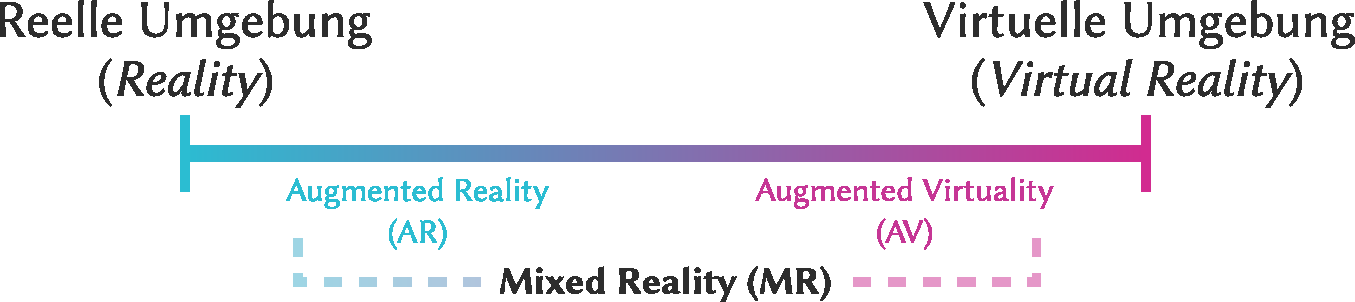
\includegraphics[width=0.9\linewidth]{figures/rv_kontinuum_milgram.pdf}}
    \caption{Das Realität-Virtualität-Kontinuum nach \textcite{Milgram1994}. Je nach Anwendung wird die Realität mehr und mehr mit virtuellen Objekten überlagert, bis schließlich nur noch eine virtuelle Umgebung dargestellt wird.}
    \label{fig:rv_kontinuum}
\end{figure}
Nach \textcite{Azuma1997} bezeichnet \emph{Augmented Reality} Systeme, welche die folgenden Eigenschaften besitzen:
\begin{itemize}
    \item Reale und virtuelle Inhalte werden kombiniert. Häufig werden hierfür virtuelle Objekte auf die reale Umgebung überlagert.
    \item Der Nutzer kann in Echtzeit mit den Systemen interagieren. So zählen z.B. Spezialeffekte in Filmen \emph{nicht} als AR.
    \item Die Inhalte werden dreidimensional mit der Umgebung registriert. Demnach ist ein 2D-Interface vor einer realen Umgebung \emph{kein} AR, selbst wenn es interaktiv ist.
\end{itemize}
AR selbst lässt sich dabei noch in die Kategorien \emph{Spatial AR} und \emph{See-Through AR} einteilen.
Bei Spatial AR werden digitale Informationen direkt in die Umgebung des Nutzers projiziert, z.B. mit einem Projektor auf einen Tisch.
Beim See-Through AR hingegen werden Displays genutzt, die entweder ein Live-Video der Umgebung zeigen oder aber transparent und damit durchsichtig sind.
Dies können See-Through HMDs wie die HoloLens sein, aber auch Smartphones in einer entsprechenden HMD-Halterung, bei denen die Rückseitenkamera für ein Live-Bild der Umgebung genutzt wird.
Hier werden die virtuellen Informationen direkt auf dem Display überlagert \autocite{Zachmann2015}.

Bei der \emph{Augmented Virtuality} (AV) werden umgekehrt reale Informationen in eine virtuelle Umgebung eingebettet.
Als Beispiel nennt \textcite[6]{Schroeder2017} die Wetterkarte im Fernsehen, bei der eine \emph{virtuelle} Karte \emph{reale} Wetterinformationen darstellt und um einen \emph{realen} Moderator erweitert wird.
%Es sei darauf hingewiesen, dass in diesem Beispiel die Interaktion zwischen dem Moderator und der Karte besteht, nicht etwa zwischen dem Zuschauer und der Karte.

\emph{Virtual Reality} ist die Bezeichnung für Anwendungen, die sich komplett in einer virtuellen Umgebung abspielen.
Um VR von herkömmlichen Computersimulationen abzugrenzen nennt \textcite{Zachmann2015} die intuitive Echtzeit-Interaktion als ein wichtiges Kriterium.
Dabei können Nutzer mit der virtuellen Umgebung über Eingabegeräte wie z.B. Controller mit sechs Freiheitsgraden (6DOF) oder haptischen Eingabegeräten interagieren.
Ein weiteres wichtiges Kriterium ist die Immersion.
Diese ergibt sich aus der Summe der vom System stimulierten und gleichzeitig abgeschirmten Sinne.
Aus diesem Grund werden bei VR-Anwendungen häufig HMDs eingesetzt, da diese gleichzeitig den Sehsinn vor der Außenwelt abschirmen und mit virtuellen Bildern stimulieren können.
Aber auch halb-immersive Displays wie eine \emph{Cave}, eine \emph{Powerwall} oder ein Volumendisplay sind möglich \parencite{Zachmann2015b}.

\textcite{Milgram1994} nennen ebenfalls den Begriff der \emph{Mixed Reality} (MR).
Dieser wird in der Literatur als Oberbegriff sowohl für AR als auch AV verwendet.
Der Begriff hebt die Kombination von realen und virtuellen Inhalten hervor.

% ===================
% KATEGORISIERUNG
% ===================

\section{Ansätze zur virtuell unterstützten Navigation}
Im Rahmen dieser Arbeit wurde in der Literatur zur AR-/VR-unterstützten Navigation recherchiert.
Die untersuchten Forschungsbeiträge lassen sich in vier Kategorien einteilen, welche in den folgenden Abschnitten mit ihren Vor- und Nachteilen beschrieben werden.

\subsection{Die \enquote{World-in-Miniature}}
\begin{figure}[ht]
    \centering
    \imagebox{
        \hfill
        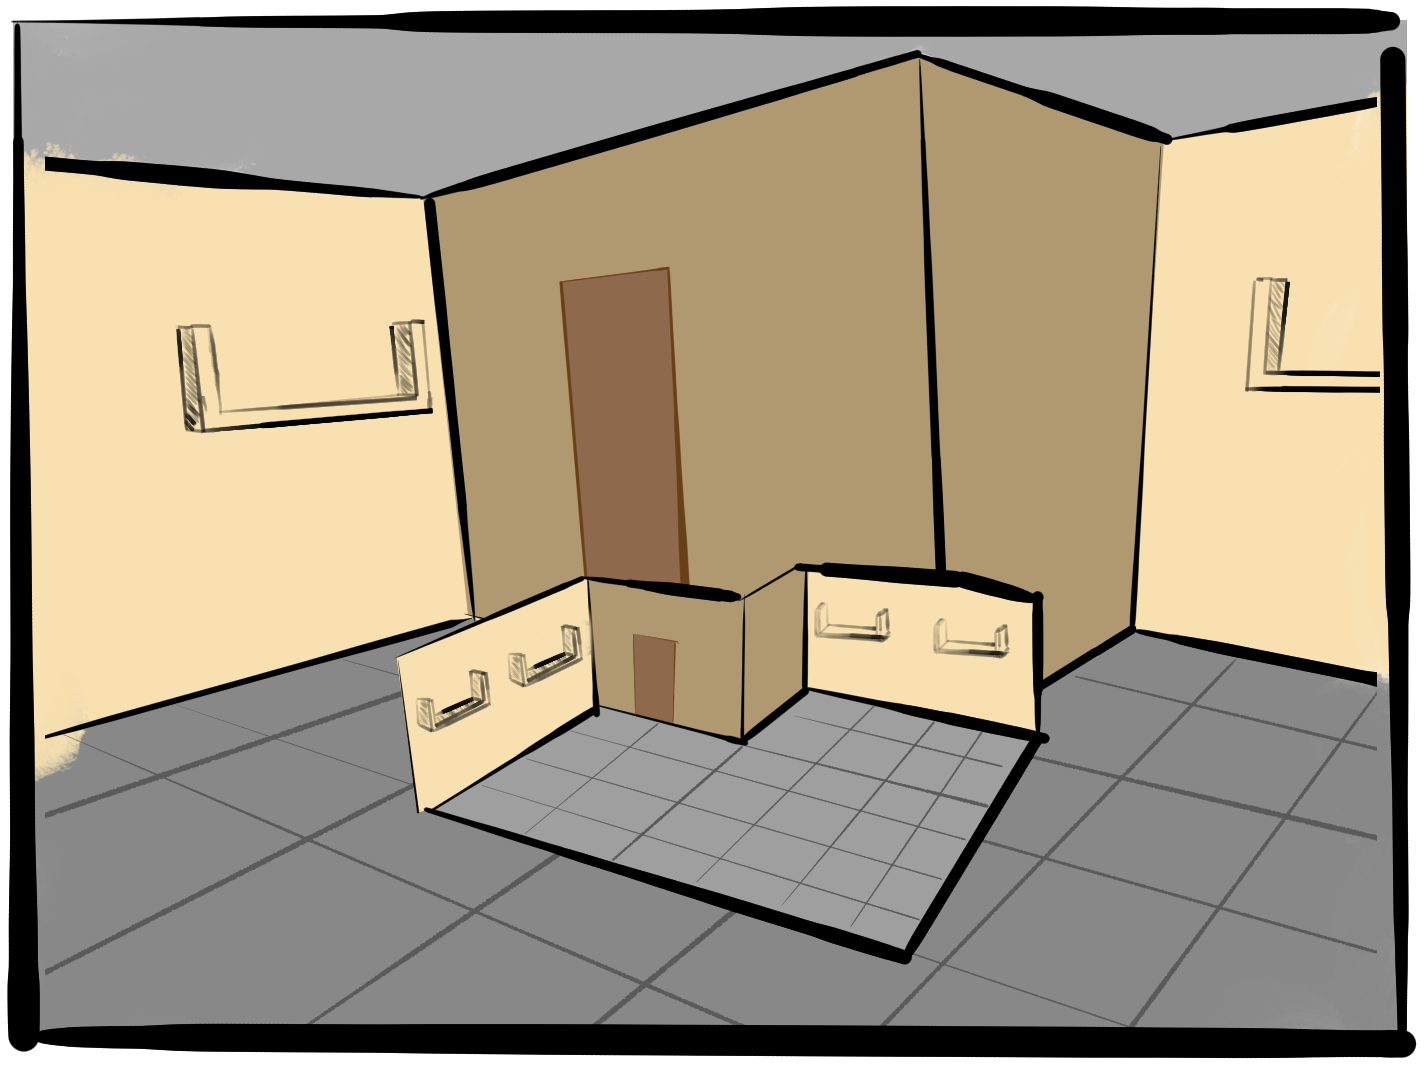
\includegraphics[height=0.4\textheight]{figures/sketch_wim.png}
        \hfill
    }
    \caption{Kategorie 1 --- Eine \enquote{World-in-Miniature} wird in der Umgebung angezeigt. (Nach \textcite[265]{Stoakley1995})}
    \label{fig:sketch_wim}
\end{figure}

Die erste Kategorie umfasst Arbeiten, welche die \emph{World-in-Miniature}-Metapher (WIM) umsetzen.
Dabei wird die nähere Umgebung miniaturisiert dargestellt und häufig als eigenständiges Objekt vom Nutzer in der Hand gehalten (siehe \autoref{fig:sketch_wim}).
Je nach Anwendung ergeben sich hieraus unterschiedliche Interaktionsmöglichkeiten \parencite{Stoakley1995}.
WIM wird z.B. eingesetzt, um die Bewegung und Interaktion in weitläufigen virtuellen Umgebungen zu vereinfachen \parencites[vgl.]{Trueba2010}{Elvezio2017}.
Da in VR die Umgebung bereits virtuell existiert, ist eine verkleinerte Variante als WIM einfach umzusetzen.

\textcite{Chittaro2005} nutzen das Konzept von WIM für mehrstöckige Gebäude als eine \emph{BreakAway}-Karte (siehe \autoref{fig:chittaro2005_breakaway}).
Hier können einzelne Stockwerke zur Seite geschoben und ausgeblendet werden, um so auf Stockwerke blicken zu können, auf denen sich der Nutzer selbst gar nicht befindet.
In einer späteren Arbeit untersuchen \textcite{Chittaro2006} 2D- und 3D-Karten als Navigationshilfe für mehrstöckige Gebäude (siehe \autoref{fig:chittaro2006_maps}).
Dabei bewegen sich die Nutzer durch ein virtuelles Gebäude von einem Zielobjekt zu einem anderen.
Die Autoren stellen fest, dass für die reine Navigation zwischen zwei Punkten eine 2D-Karte effektiver ist.
Allerdings baut sich die räumliche Vorstellung der Objekte im Gebäude in beiden Darstellungen gleichermaßen auf.

\textcite{Li2013} untersuchen ebenfalls die Auswirkungen von 2D- und 3D-Dar\-stel\-lun\-gen bei der Navigation mehrstöckiger Gebäuden.
Satt einer detaillierten Karte wird hier nur eine strukturelle Karte (Flur und Treppen) gezeigt.
Im Fall der 3D-Karte rotiert die Ansicht automatisch, wenn die Nutzer sich bewegen.
Das Ergebnis der Autoren ist, dass sich beide Darstellungen gleichermaßen zum Aufbau eines räumlichen Verständnisses des Gebäudes eignen.

\textcite{Vallance2001} schlagen zudem eine Krümmung der WIM-Umgebung vor, um so ein Verdecken durch Wände und andere Objekte zu minimieren.

Außerhalb der VR sind WIM-Anwendungen ebenfalls möglich.
\textcites{Mulloni2011a}{Mulloni2012} präsentieren eine See-Through-AR-Anwendung kombiniert aus AR-Hinweisen und WIM.
Während Nutzer durch ein Gebäude navigieren werden AR-Pfeile sowie Navigationsanweisungen in Form von \enquote{Aktivitäten} auf einem Smartphone angezeigt (\autoref{sfig:mulloni2011_wim_b}, \subref{sfig:mulloni2011_wim_e}).
Sobald zuvor platzierte Poster an Infopunkten im Gebäude erreicht und gescannt werden, wechselt die Ansicht zu einer WIM-Darstellung der Etage mit der hervorgehobenen Route zum Zielort (\autoref{sfig:mulloni2011_wim_a}, \subref{sfig:mulloni2011_wim_c}, \subref{sfig:mulloni2011_wim_d}).
Die WIM-Übersicht hilft Nutzern, Orientierungspunkte (\emph{\enquote{Landmarks}}) in der Umgebung wiederzuerkennen, was zu weniger Fehlern bei der Navigation führt.

\begin{figure}
    \begin{subfigure}{.49\textwidth}
        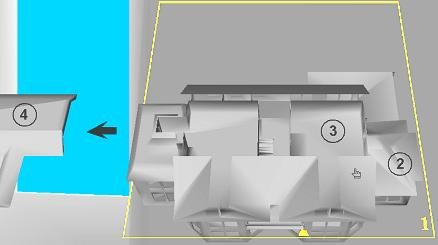
\includegraphics[width=\textwidth]{figures/chittaro2005_breakaway_a.png}
%        \caption{}
    \end{subfigure}
    \hfill
    \begin{subfigure}{.49\textwidth}
        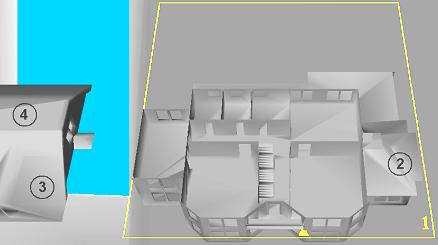
\includegraphics[width=\textwidth]{figures/chittaro2005_breakaway_b.png}
%        \caption{}
    \end{subfigure}
    \caption{In der \emph{\enquote{Examine View}} der BreakAway-Karte können Stockwerke zur Seite geschoben werden, um den Blick auf darunterliegende Stockwerke zu ermöglichen. \quelle{\cite{Chittaro2005}}}
    \label{fig:chittaro2005_breakaway}
\end{figure}

\begin{figure}
	\centering
	\begin{subfigure}{0.49\textwidth}
		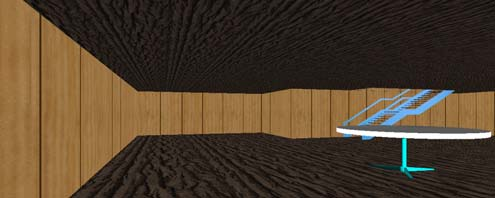
\includegraphics[width=\textwidth]{figures/chittaro2006_ve.png}
		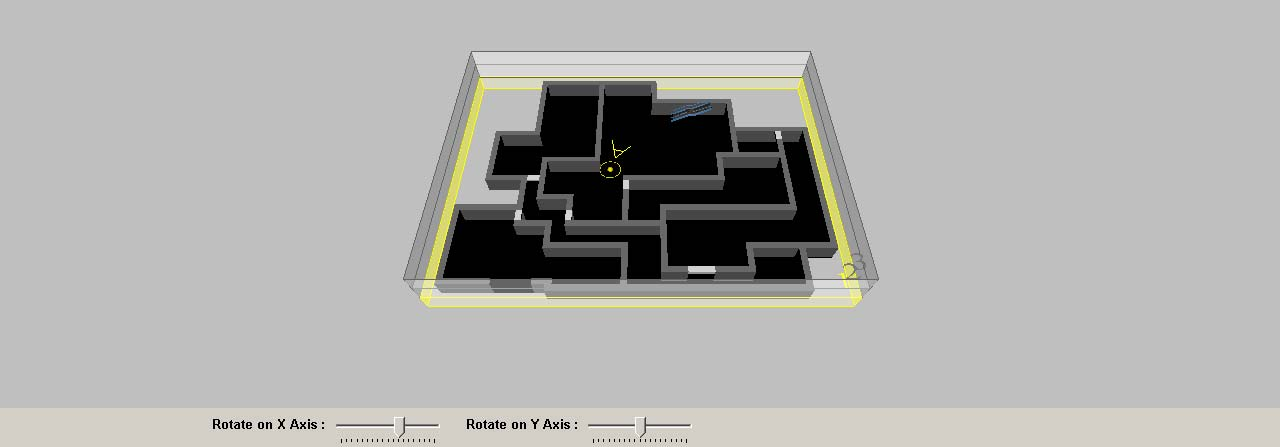
\includegraphics[width=\textwidth]{figures/chittaro2006_3dm.png}
		\caption{}
		\label{sfig:chittaro2006_3dm}
    \end{subfigure}
    \hfill
	\begin{subfigure}{0.49\textwidth}
		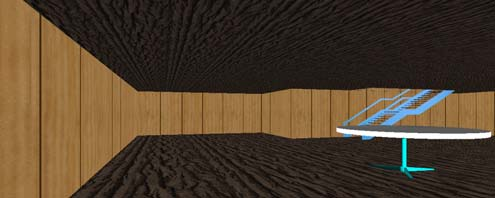
\includegraphics[width=\textwidth]{figures/chittaro2006_ve.png}
		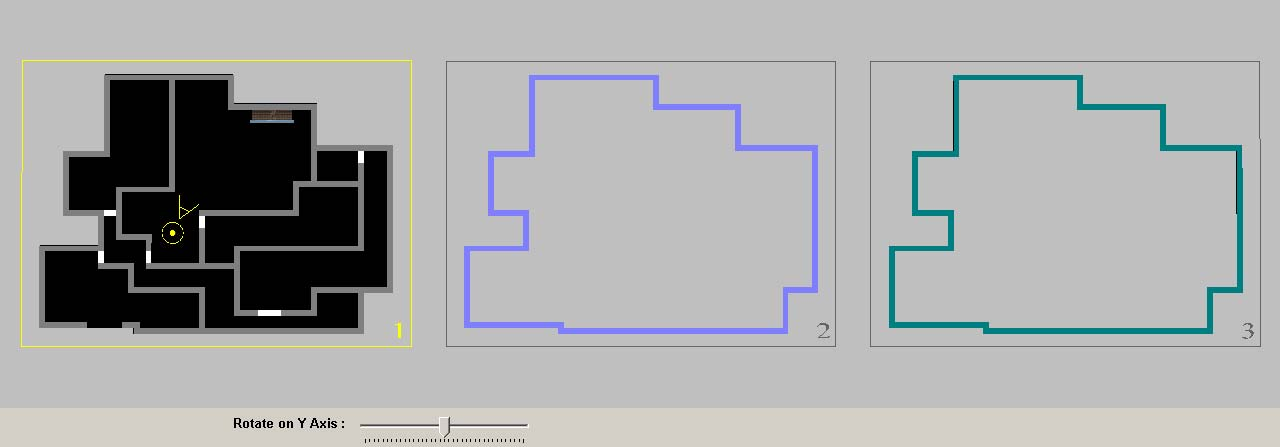
\includegraphics[width=\textwidth]{figures/chittaro2006_2dm.png}
		\caption{}
		\label{sfig:chittaro2006_2dm}
	\end{subfigure}
	\caption{Navigation eines virtuellen Gebäudes. Eine 3D-Karte \subref{sfig:chittaro2006_3dm} oder eine 2D-Karte \subref{sfig:chittaro2006_2dm} unterstützen die Navigation. \quelle{\cite[230]{Chittaro2006}}}
	\label{fig:chittaro2006_maps}
\end{figure}

\begin{figure}
    \begin{subfigure}{.18\textwidth}
        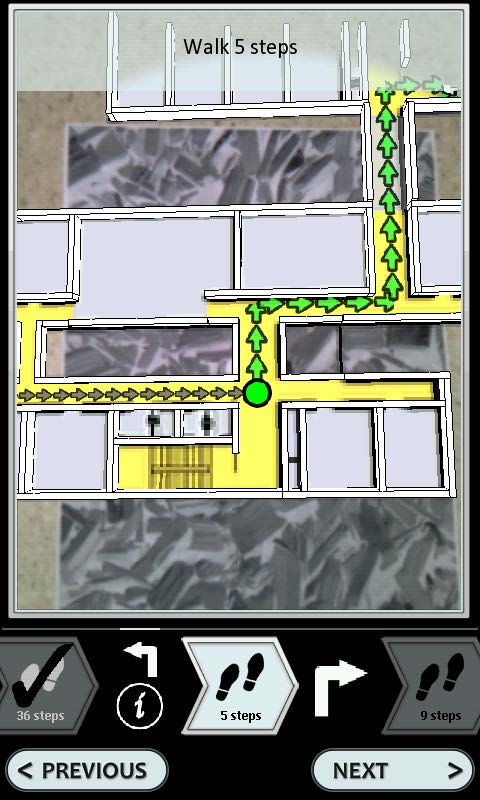
\includegraphics[width=\textwidth]{figures/mulloni2011_wim_a.png}
        \caption{}
        \label{sfig:mulloni2011_wim_a}
    \end{subfigure}
    \hfill
    \begin{subfigure}{.18\textwidth}
        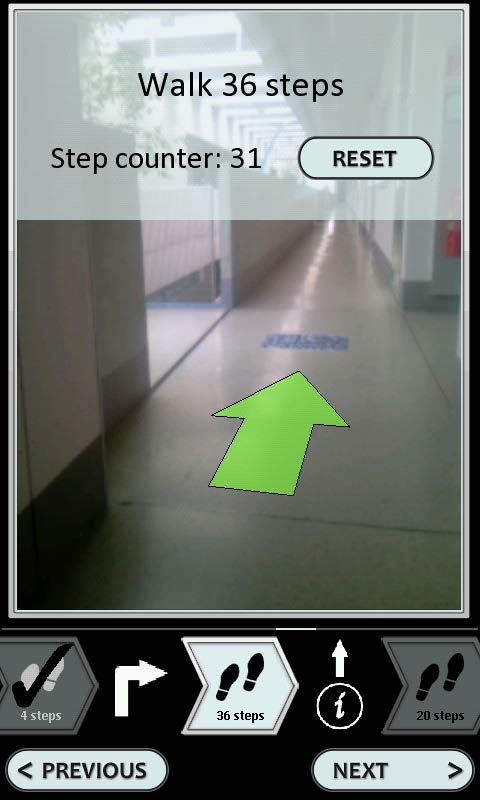
\includegraphics[width=\textwidth]{figures/mulloni2011_wim_b.png}
        \caption{}
        \label{sfig:mulloni2011_wim_b}
    \end{subfigure}
    \hfill
    \begin{subfigure}{.18\textwidth}
        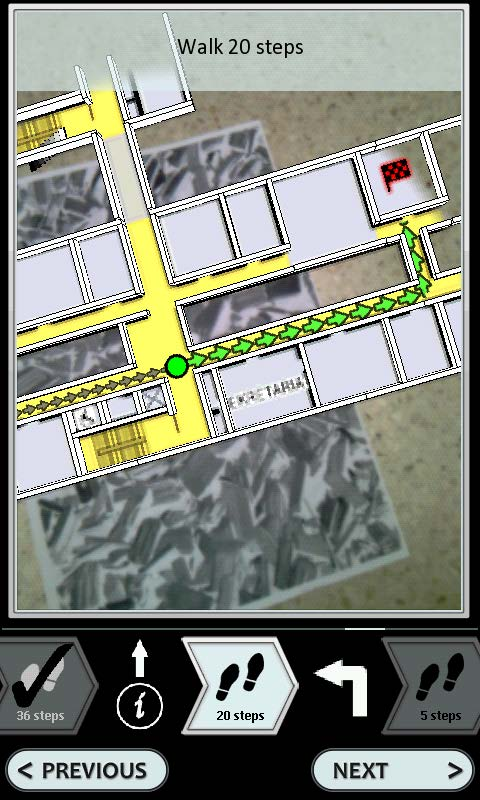
\includegraphics[width=\textwidth]{figures/mulloni2011_wim_c.png}
        \caption{}
        \label{sfig:mulloni2011_wim_c}
    \end{subfigure}
    \hfill
    \begin{subfigure}{.18\textwidth}
        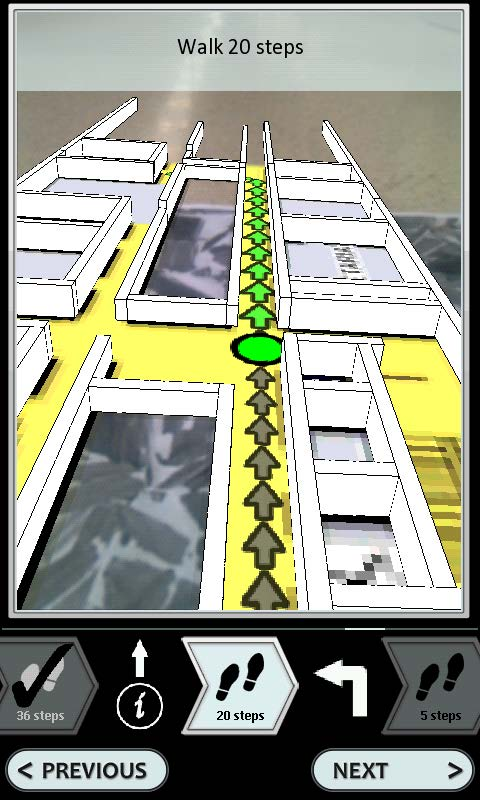
\includegraphics[width=\textwidth]{figures/mulloni2011_wim_d.png}
        \caption{}
        \label{sfig:mulloni2011_wim_d}
    \end{subfigure}
    \hfill
    \begin{subfigure}{.18\textwidth}
        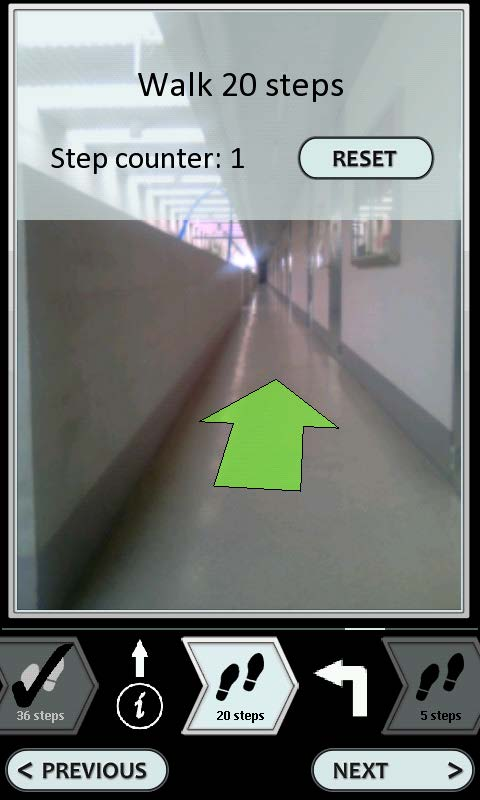
\includegraphics[width=\textwidth]{figures/mulloni2011_wim_e.png}
        \caption{}
        \label{sfig:mulloni2011_wim_e}
    \end{subfigure}
    \caption{AR-Interface für Indoor-Navigation basierend auf WIM.\@ An den Lokalisierungspunkten wird die Indoor-Karte als WIM angezeigt und mit der Position/Rotation der Umgebung registriert. \quelle{\cite{Mulloni2011}}}
    \label{fig:mulloni2011_wim}
\end{figure}

Nach \textcite[272]{Stoakley1995} ergeben sich die meisten Vorteile der WIM aus der Tatsache, dass diese sich rotieren und skalieren lässt.
So können Nutzer die Umgebungen aus mehreren Blickwinkeln betrachten und Verdeckungen durch Wände umgehen.
Ein weiterer Vorteil ist die 3D-Struktur einer WIM.
Durch die dreidimensionale Darstellung von besonderen Strukturen der Umgebung (z.B. die Wände in einem Gebäude) können Nutzern die entsprechenden Strukturen in der Umgebung schneller wiederzufinden.
Dadurch fällt Nutzern die Selbstorientierung in der Umgebung leichter \parencite[215]{Mulloni2012}.

Der größte Nachteil der WIM-Methode ist, dass vorab ein dreidimensionales Modell als WIM erstellt werden muss.
Während bei den anderen Kategorien lediglich virtuelle Objekte auf die reale Welt überlagert werden, muss für eine WIM ein virtuelles Abbild der Umgebung geschaffen werden.
Dies gilt insbesondere dann, wenn anstatt einer virtuellen Umgebung ein Szenario in der realen Welt umgesetzt wird (wie es z.B. bei \textcite{Mulloni2012} der Fall ist).
Dies bringt Schwierigkeiten mit sich.
Zum einen stellen \citeauthor{Mulloni2012} fest, dass es einen Kompromiss zwischen dem Modellierungsaufwand für das Erstellen der WIM und dem Realismus der Strukturen, die vom Nutzer wiedererkannt werden sollen, geben muss \parencite[215]{Mulloni2012}.
\citeauthor{Elvezio2017} erklärt, dass auch die korrekte Skalierung einer WIM nicht trivial zu wählen ist.
Wenn die WIM ein zu großes Modell darstellt (z.B. eine ganze Stadt), könnte dies nicht in das Sichtfeld des Nutzers passen und ein Teil des Modells würde abgeschnitten werden.
Falls die WIM zu klein ist könnte wiederum die Erkennbarkeit von Details sowie die Interaktion mit einzelnen Objekten auf der WIM erschwert werden \parencite[1]{Elvezio2017}.
\citeauthor{Stoakley1995} führt schließlich an, dass Irritationen bei Nutzern entstehen können, wenn die Beleuchtung des Modells nicht mit der der Umgebung übereinstimmt \parencite[269]{Stoakley1995}.

\subsection{Virtuelle umgebungsintegrierte Navigationshelfer}
\begin{figure}[ht]
    \centering
    \imagebox{
        \hfill
        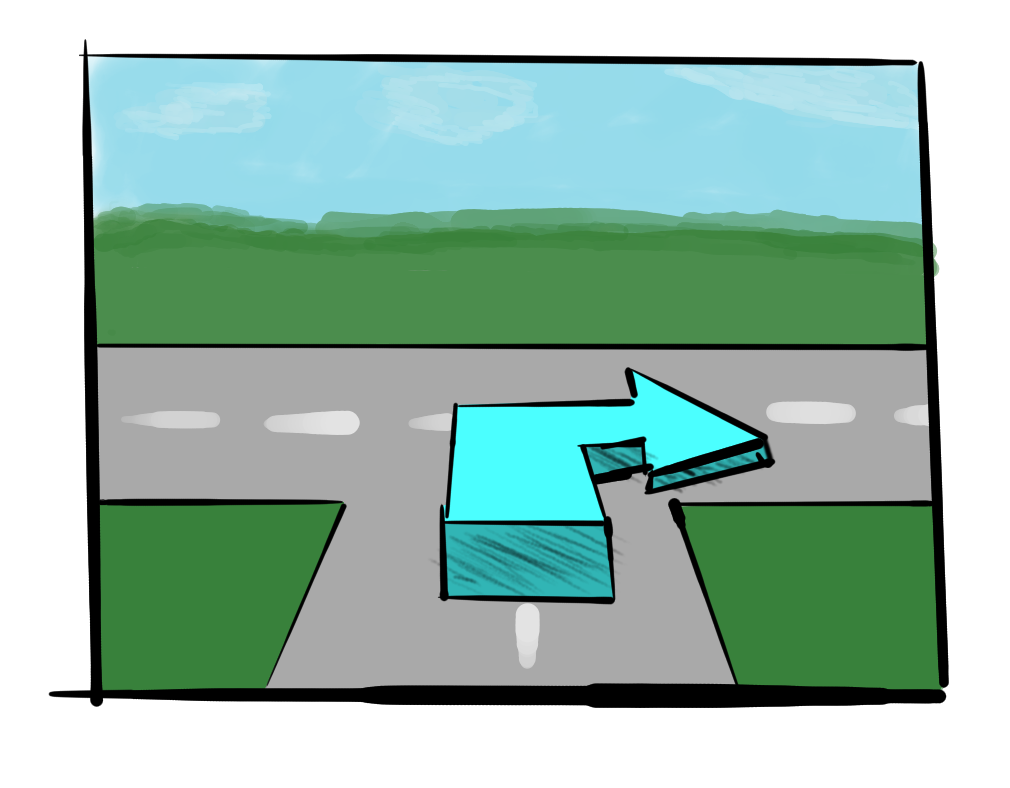
\includegraphics[height=0.4\textheight]{figures/sketch_ar_arrows}
        \hfill
    }
    \caption{Kategorie 2 --- Virtuelle Navigationshelfer (z.B. Pfeile) werden in die reale Welt verankert.}
    \label{fig:sketch_ar_arrows}
\end{figure}

Ansätze, bei denen virtuelle Objekte als Navigationshelfer mit sechs Freiheitsgraden in die Umgebung integriert werden, bilden die zweite Kategorie.
Dies wird schematisch in \autoref{fig:sketch_ar_arrows} dargestellt.
Für diese Kategorie ist der Einsatz von See-Through Displays charakterisierend.
Es lassen sich Arbeiten sowohl mit MR-HMDs als auch Handgeräte wie Smartphones als Nutzungsschnittstelle finden.

Bereits \textcite{Hoellerer1999} stellen ein AR-System vor, bei dem zwei Nutzer kooperieren können (siehe \autoref{fig:hoellerer_mars}).
Der eine Nutzer bewegt sich zu Fuß mit einem HMD und einem Tablet-Computer in der Außenwelt.
Durch das HMD können ihm augmentierte Informationen zur Umgebung und sogar ganze virtuelle Gebäude dargestellt werden, die mit der Umgebung registriert sind.
Der andere Nutzer kann entweder über ein Desktop-Interface oder eine AR-Darstellung der Karte Routen und Informationen in der Umgebung platzieren.
Damit stellt diese Arbeit eine frühe Implementierung für ein HMD dar, die sowohl Navigations- als auch Explorationsaufgaben unterstützt.
\begin{figure}
    \centering
    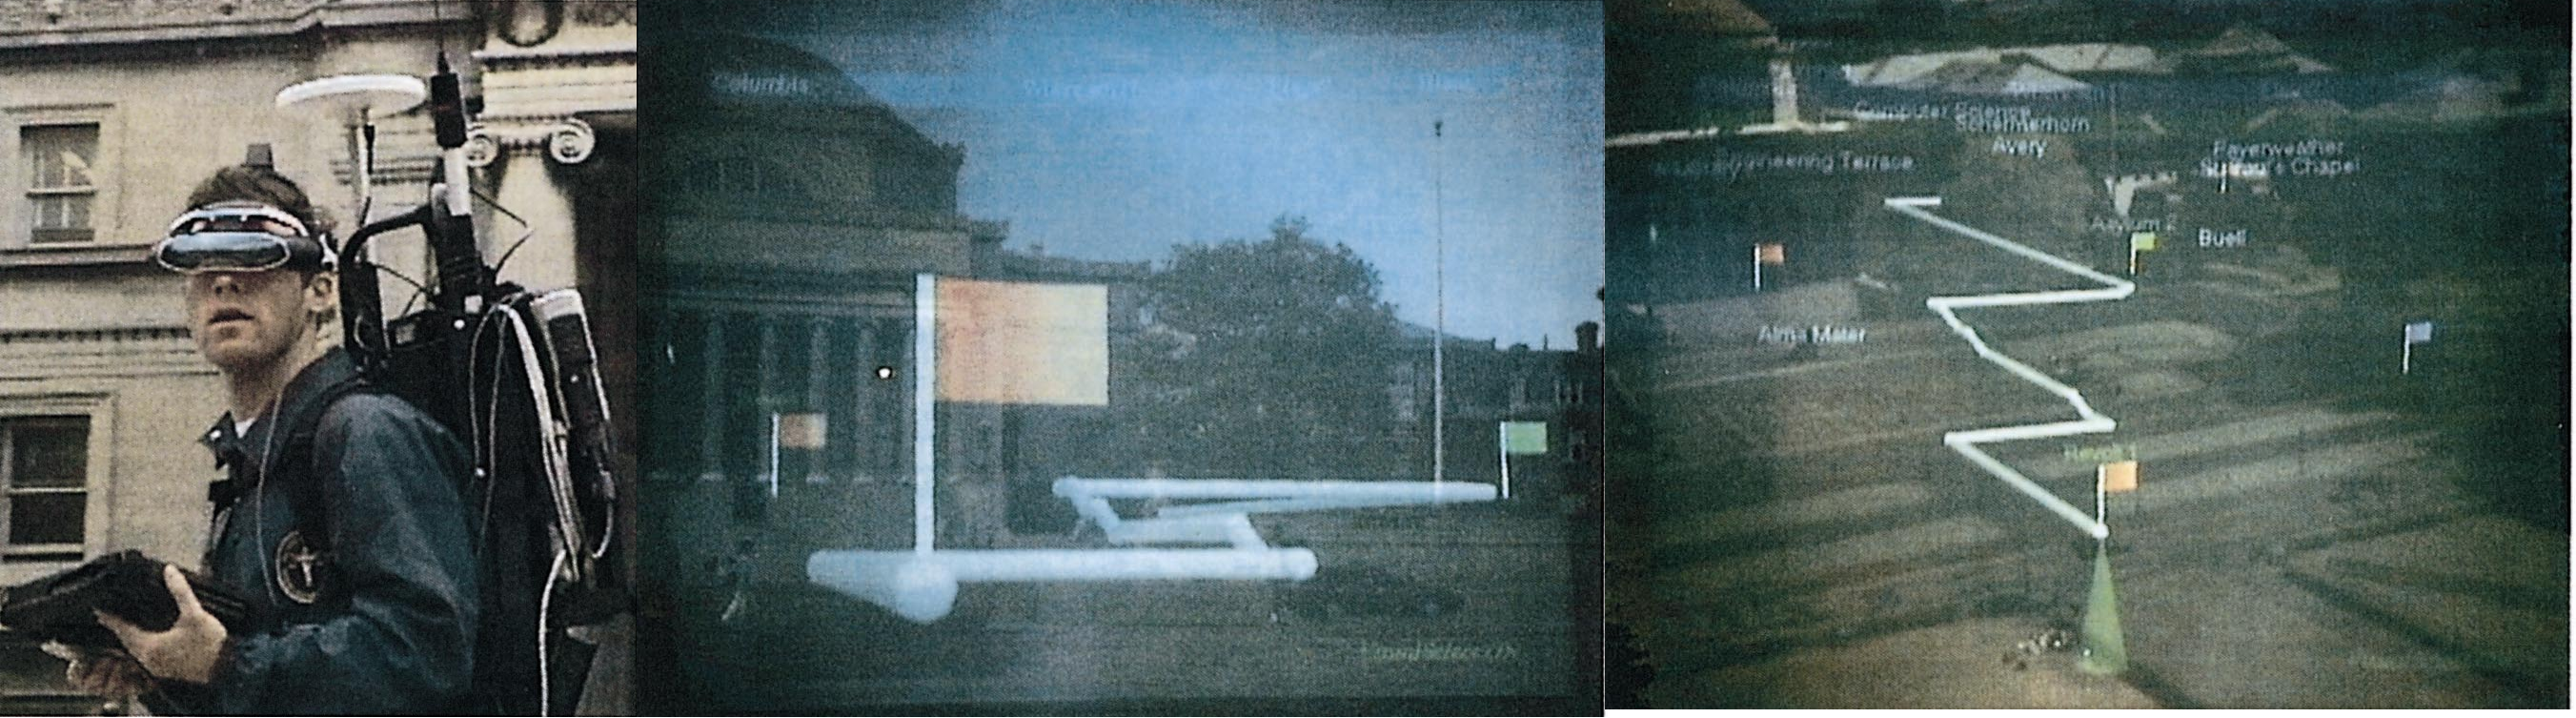
\includegraphics[width=\textwidth]{figures/hoellerer_ar_mars}
    \caption{Dem HMD-Nutzer wird in seiner Umgebung ein virtueller Pfad sowie Informationen zu den Gebäuden angezeigt. \quelle{\cite{Hoellerer1999}}}
    \label{fig:hoellerer_mars}
\end{figure}

\textcite{Reitmayr2004} erweitern diesen Ansatz um ein \emph{Extensible Markup Language} Datenmodell (XML-Datenmodell) zur Speicherung von Gebäudegeometrie, -informationen und Wegpunkten.
Nutzer können dadurch Informationen zu einzelnen Gebäudeabschnitten erhalten.
Weiterhin wird für die virtuellen Pfade durch die geometrischen Modelle die Verdeckung durch Gebäude korrekt berechnet.
Das bedeutet, dass für Nutzer Pfade nicht sichbar sind, wenn diese hinter Gebäuden entlang verlaufen (siehe \autoref{fig:reitmayr2004_path}).

Ein weiterer, wichtiger Gegenstand der Forschung ist die virtuell unterstütze Navigation beim Autofahren.
Hier ist die korrekte Navigation wichtig und Fehler können im Ernstfall fatale Folgen haben \parencite{Lin2017}.
Ein häufig eingesetztes Mittel zur Verbesserung der Navigation ist die virtuelle Hervorhebung der Straßenführung.
\textcite{Narzt2006} präsentieren ein allgemeines Framework zur Darstellung einer virtuellen Route.
Das Framework kann sowohl für Fahrzeug- als auch Fußgängernavigation und auf verschiedenen Endgeräten eingesetzt werden.
Für den Einsatz im Auto schlagen die Autoren die Windschutzscheibe als Display vor.
Dadurch wäre das AR-Display in der natürlichen Umgebung des Nutzers integriert.

\textcite{Bark2014} erweitern diesen Ansatz.
Sie ersetzen in einem zuvor aufgenommenen Video den statischen, virtuell eingefügten Pfad durch eine Reihe animierter Papierflieger, die entlang der geplanten Route fliegen.
\textcite{Kim2009} präsentieren eine 2.5D-Karte mithilfe eines Fahrsimulators.
Von der Oberseite der Windschutzscheibe schiebt sich eine 2D-Karte ins Sichtfeld, die sich nach und nach dreidimensional mit der Straße verbindet.
Bei beiden Ansätzen wiesen die Autoren beim Vergleich mit einem herkömmlichen \emph{top-down} GPS-System nach, dass die Probanden dem Straßenverlauf durch die AR-Unterstützung besser folgen konnten und weniger Fehler bei der Navigation machten.

\begin{figure}
\begin{minipage}[t]{0.48\textwidth}
    \centering
    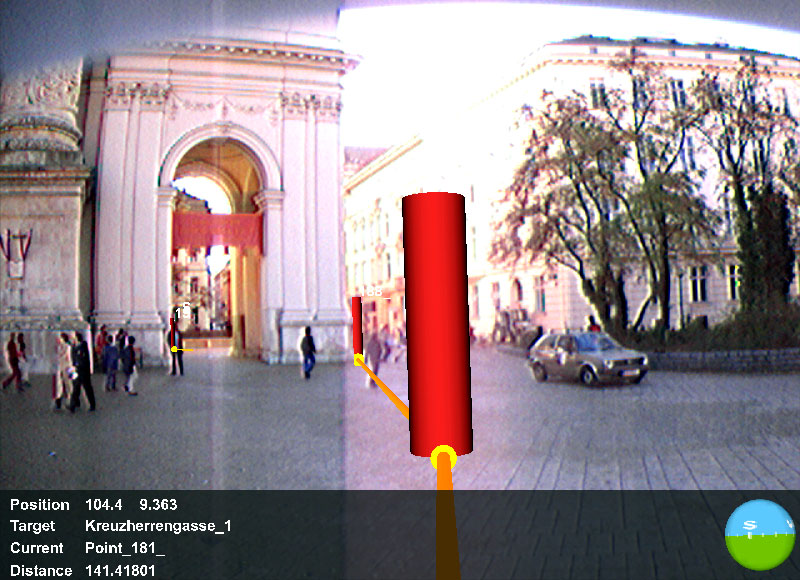
\includegraphics[width=\textwidth, height=5cm]{figures/reitmayr2004_path}
    \caption{Virtueller Pfad hebt die Route zum ausgewählten Zielobjekt hervor und wird durch Gebäude verdeckt. \quelle{\cite{Reitmayr2004}}\hfill}
    \label{fig:reitmayr2004_path}
\end{minipage}%
\hfill
\begin{minipage}[t]{0.48\textwidth}
    \centering
    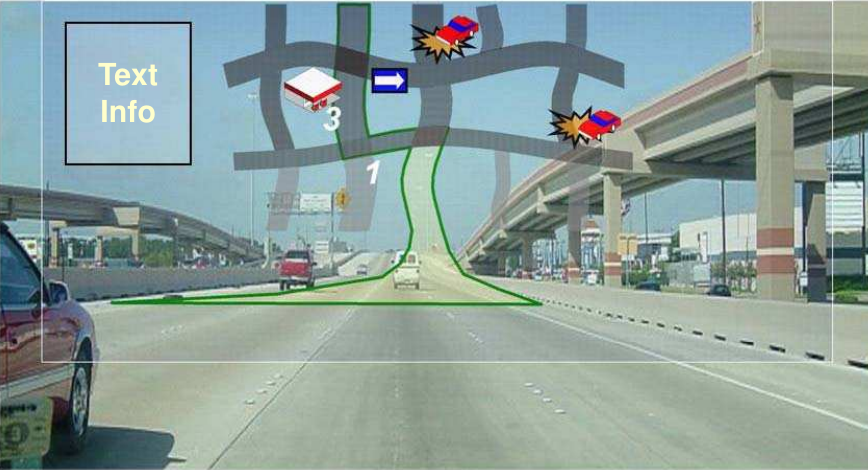
\includegraphics[width=\textwidth, height=5cm]{figures/kim2009_concept_2_5d_map}
    \caption{Konzept einer AR-2.5D-Karte: 2D-Karte schiebt sich vom oberen Bildschirmrand hinunter und \enquote{verschmilzt} mit Straßenführung. \quelle{\cite{Kim2009}}\hfill}
    \label{fig:kim2009_2_5d_map}
\end{minipage}
\end{figure}

Ein Vorteil dieser Herangehensweisen ist, dass die Hände durch die Verwendung eines MR-HMDs oder eines Windschutzscheibendisplays frei bleiben.
Dadurch haben Nutzer die möglichkeit, Controller oder Fahrzeuge zu bedienen, Gestensteuerung durchzuführen oder direkt mit der Umgebung zu interagieren.

Außerdem bleibt die Umgebung durch das See-Through-Display weiterhin sichtbar.
So wird der Fokus der Nutzer nicht von der Umgebung auf das Ausgabegerät gelenkt.
Dies ist vor allem für mobile Szenarios von Vorteil, bei denen längere Strecken zurückgelegt werden und eine höhere Anzahl an Gefahrenstellen (Verkehr, schwierige Straßenführung, etc.) zu erwarten ist.

Eine Herausforderung (und damit auch ein Nachteil) dieser Variante ist die erforderliche Präzision zur Positionierung der Navigationshelfer.
Wie \citeauthor{Wiesner2017} und \citeauthor{Pfannmueller2015} ausführen, reicht die Präzision von Satellitensystemen wie dem \emph{Global Positioning System} (GPS) nicht aus, um virtuelle Objekte ohne Abweichung im Bereich von mehreren Metern zu platzieren.
Dies führt in der Folge zu mehr Navigationsfehlern \parencites[378]{Wiesner2017}{Pfannmueller2015}.
Als Alternative kann die 3D-Rekonstruktionsfunktion eines MR-HMDs wie der HoloLens genutzt werden, um eine dreidimensionale Punktwolke der Szene zu erhalten und so den Navigationshelfer in einem lokalen Referenzrahmen zu platzieren.
\citeauthor{Schroeder2017} weist allerdings darauf hin, dass die HoloLens bei normalem Tageslicht kaum bis gar nicht verwendbar ist, da die dargestellten Bilder nicht zu erkennen sind und die Sensoren die 3D-Struktur nicht korrekt analysieren \parencite[47]{Schroeder2017}.
Ähnliches stellt \citeauthor{Strange2018} für die MagicLeap fest.
Dies schränkt die Möglichkeiten ein, virtuelle Navigationshelfer mit aktuell verfügbarer Technologie in die Umgebung zu integrieren.

\subsection{\enquote{Magische Lupe} augmentiert physische Karte}
\begin{figure}[h]
    \centering
    \imagebox{
        \hfill
        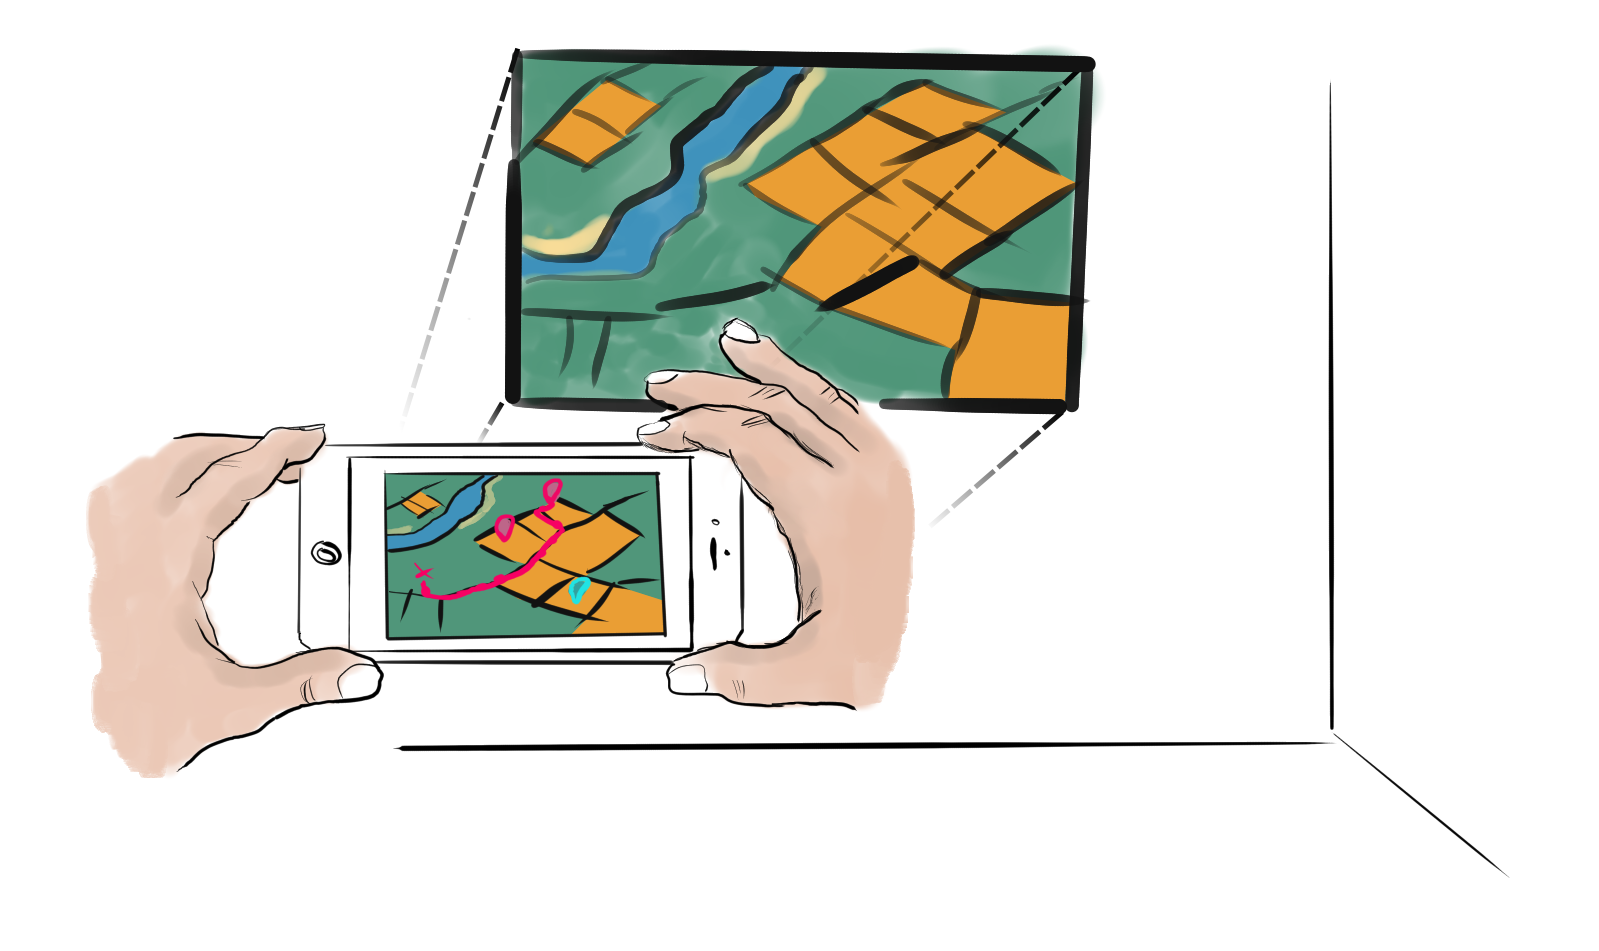
\includegraphics[height=0.4\textheight]{figures/sketch_ar_physical}
        \hfill
    }
    \caption{Kategorie 3: Physische Karten werden durch virtuelle Inhalte (hier \textcolor{magenta}{Magenta} und \textcolor{cyan}{Türkis}) angereichert.}
    \label{fig:sketch_ar_physical}
\end{figure}

Ähnlich wie vorigen Abschnitt beschrieben wird in der dritten Kategorie die Realität um digitale Informationen durch See-Through-AR erweitert.
Jedoch werden die virtuellen Informationen in diesem Fall im Kontext \emph{einzelner physischer Objekte} angezeigt.
Die Skizze in \autoref{fig:sketch_ar_physical} stellt das Prinzip dar.
Arbeiten, die dieser Kategorie zugeordnet werden, bedienen sich Bildausgabegeräten (Displays), die gleichzeitig über Kameratechnologie verfügen.
Sie setzen damit die \enquote{Magische Lupe}-Metapher (\emph{Magic Lens}) um, bei der das Handgerät (wie z.B. ein Smartphone) wie eine Lupe über einem physischen Objekt entlanggeführt wird, um so neue Informationen hervorzubringen.
Die virtuellen Informationen befinden sich effektiv auf einer transparenten Ebene vor dem Objekt und werden durch das Display des Handgeräts sichtbar gemacht \parencite{Bier1994}.
Mit den Kameras und entsprechenden Bildverarbeitungsverfahren können einzelne physische Objekte getrackt werden.
Zur Unterstützung dieser Verfahren werden oft spezielle Markierungen verwendet, die sich von der Umgebung abgheben und besser verfolgt werden können.

Ein Vertreter dieser Kategorie ist die Arbeit von \textcite{Rohs2009}.
Die Autoren implementieren auf einem Kamerahandy die virtuelle Anzeige von Parkplatz-Kosten vor dem Hintergrund einer physischen Karte (siehe \autoref{fig:rohs2009_ar_map}).
Sie stellen fest, dass Nutzer mit der Magischen Lupe die gesuchten Parkplätze schneller finden, umso niedriger die Dichte der anzuzeigenden Informationen ist.
Bei einer hohen Dichte sind die zu suchenden Informationen bereits auf dem Display zu sehen, weswegen ein Fokussieren der physischen Karte keinen Mehrwert bringt.

Die gleiche Technik verwenden auch \textcite{Morrison2009}.
Hier wird die Augmentierung einer Papierkarte für ein ortsbezogenes Spiel eingesetzt (siehe \autoref{fig:morrison2009_ar_game}).
Während ein Teil der Gruppen die Magische AR-Lupe verwendet, nutzt der andere Teil herkömmliche 2D-Kartennavigation.
Die Autoren entdecken, dass durch die Interaktion mit der Magischen Lupe kollaborative Elemente der Gruppen gefördert werden.
Dazu gehören Kommunikation, Diskussion und Rollentausch.

\begin{figure}[h]
\begin{minipage}[t]{0.48\textwidth}
    \centering
    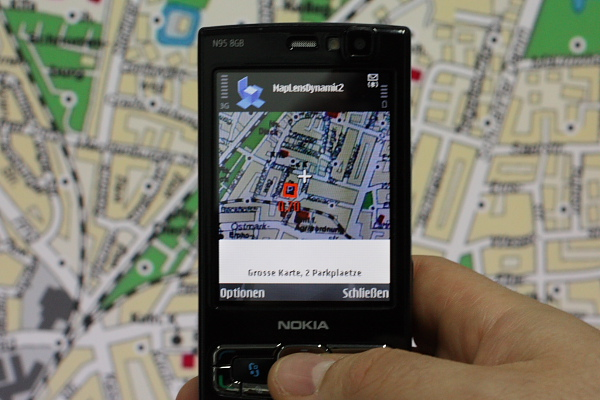
\includegraphics[width=\textwidth, height=0.25\textheight]{figures/rohs2009_ar_map.png}
    \caption{%
        Eine physische Karte wird mittels eines Kamerahandys um Preise für Parkplätze angereichert.
        \quelle{\cite{Rohs2009}}
    }
    \label{fig:rohs2009_ar_map}
\end{minipage}%
\hfill
\begin{minipage}[t]{0.48\textwidth}
    \centering
    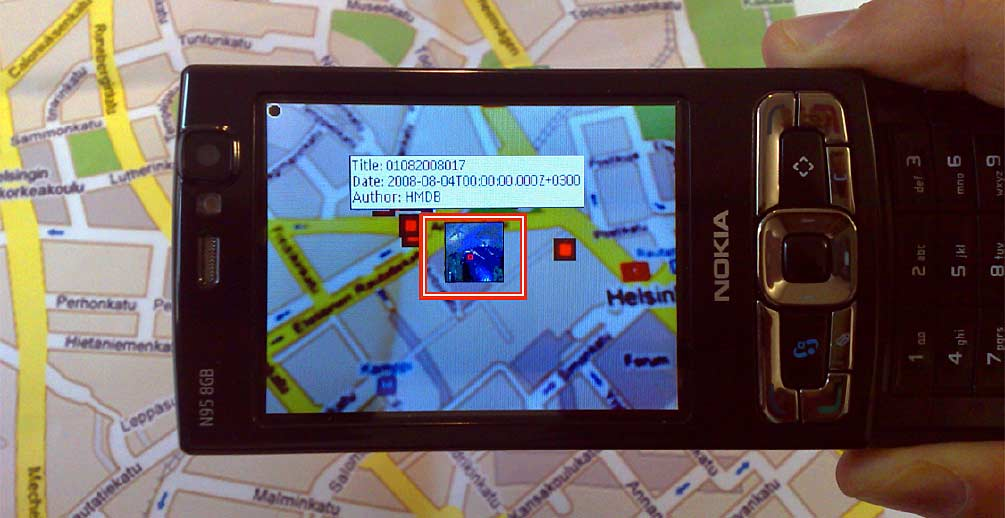
\includegraphics[width=\textwidth, height=0.25\textheight]{figures/morrison2009_ar_game.png}
    \caption{%
        Mit \enquote{MapLens} wird eine Papierkarte virtuell erweitert. %
        Über das rote Quadrat lassen sich augmentierte Icons (rote Punkte) auswählen. %
        \quelle{\cite{Morrison2009}}
    }
    \label{fig:morrison2009_ar_game}
\end{minipage}
\end{figure}

Auch \textcite{Wiehr2017} setzen die Magische AR-Lupe als kollaboratives Werkzeug ein (siehe \autoref{fig:wiehr2017_artopos}).
Mehrere Nutzer können mit Smartphones topologische Papierkarten als 3D-Landschaft darstellen lassen und gemeinsam Routen durch die Landschaft planen.

Zu dieser Kategorie gehört auch der Ansatz von \textcite{Moore2005}.
Die Autoren nutzen eine Webcam sowie einen physischen Würfel mit Markern, um digitale Karten auf die Würfelseiten zu überlagern.
Durch Rotation des Würfels kann ein angrenzender Kartenabschnitt angezeigt werden.
Somit nutzen die Autoren den Würfel als taktile Nutzungsschnittstelle für diese AR-Kartenanwendung.

\begin{figure}[h]
\begin{minipage}[t]{0.48\textwidth}
    \centering
    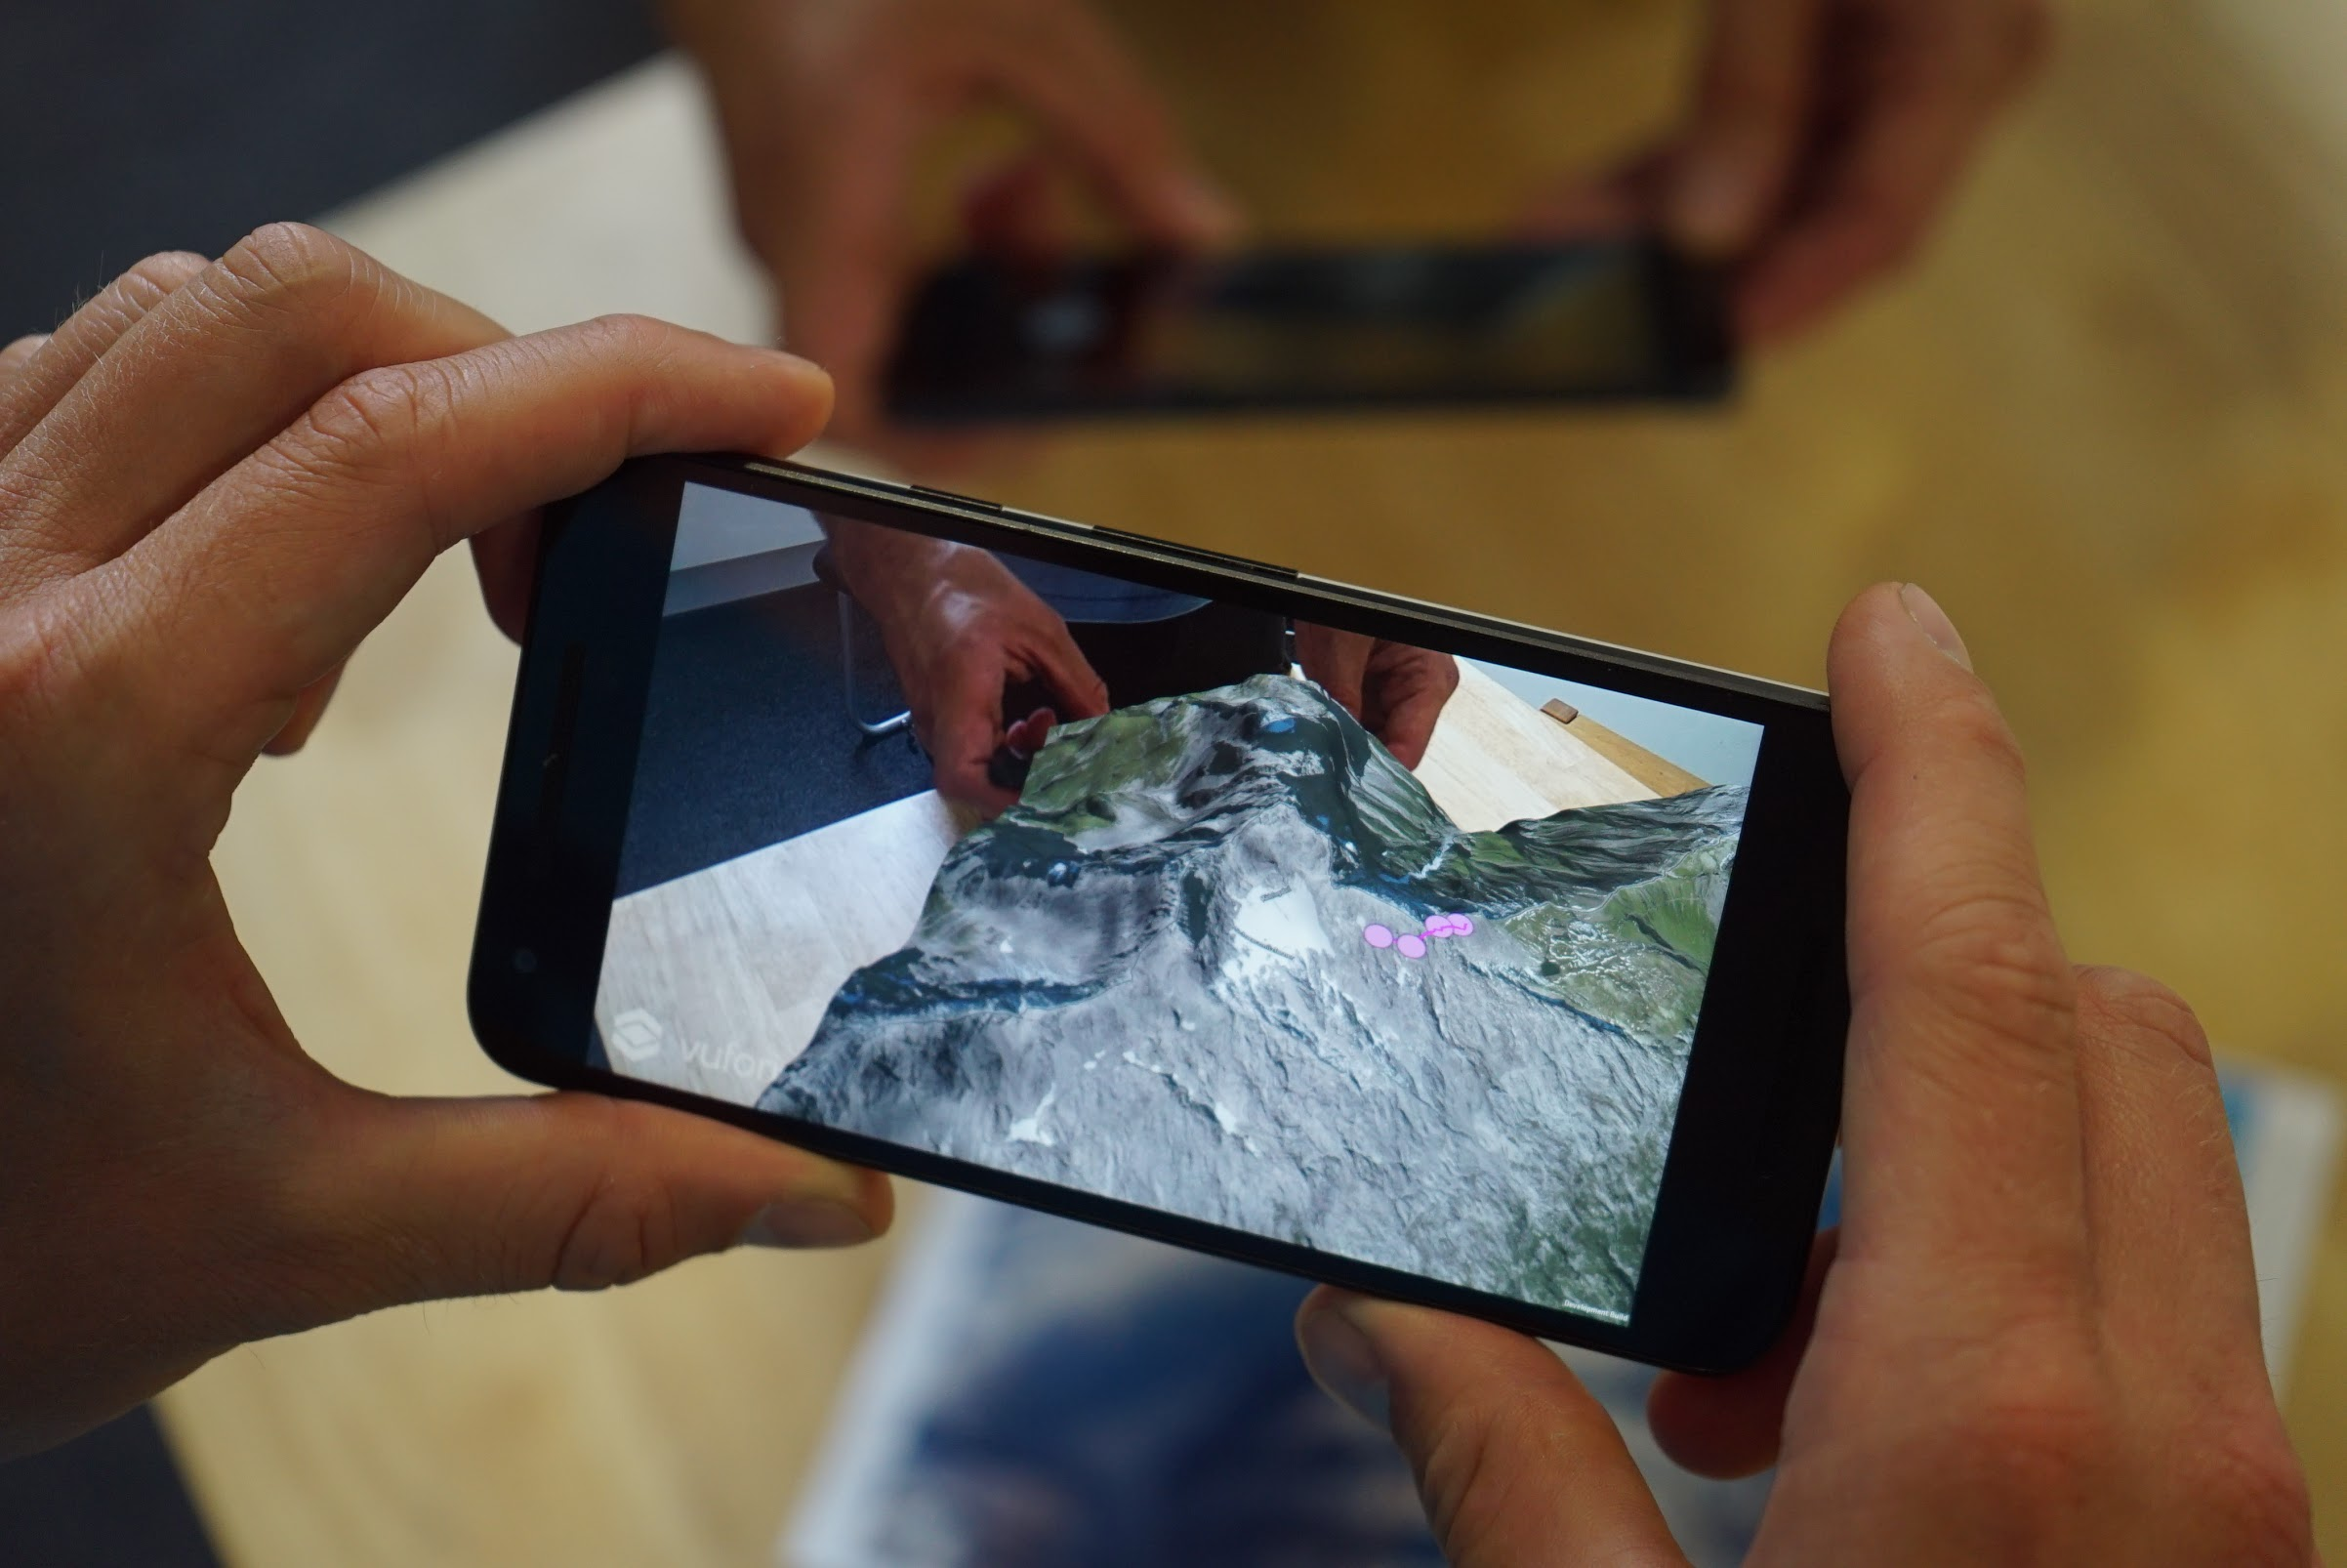
\includegraphics[width=\textwidth, height=0.25\textheight]{figures/wiehr2017_artopos.png}
    \caption{%
        Mit \emph{ARTopos} wird eine topologische Papierkarte augmentiert, um kollaborativ Routen zu planen. %
        \quelle{\cite{Wiehr2017}}
    }
    \label{fig:wiehr2017_artopos}
\end{minipage}
\hfill
\begin{minipage}[t]{0.48\textwidth}
    \centering
    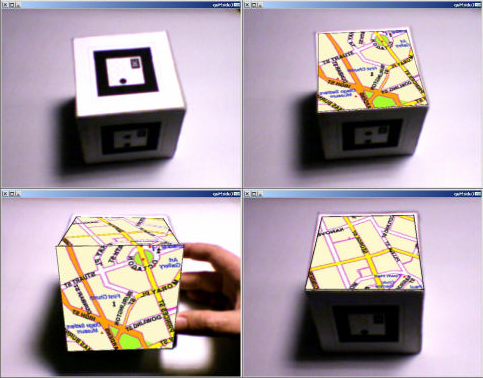
\includegraphics[width=\textwidth, height=0.25\textheight]{figures/moore2005_cube.png}
    \caption{%
        Ein Würfel wird über Marker und Webcam augmentiert. %
        Das Rotieren des Würfels ändert den Kartenausschnitt. %
        \quelle{\cite{Moore2005}}
    }
    \label{fig:moore2005_cube}
\end{minipage}%
\end{figure}

% TODO: Mehr Vor-/Nachteile?
Ein Vorteil dieser Ansätze ist, dass keine MR-HMDs benötigt werden, um die virtuellen Inhalte in der Szene zu platzieren.
Für die Verfahren werden herkömmliche Farbkameras und Displays eingesetzt, was die technischen Anforderungen gegenüber der vorigen Kategorie reduziert.

Beim Ansatz der Magischen Lupe sind jedoch die Hände durch das jeweilige Handgerät belegt, was eine gleichzeitige Interaktion mit der Umgebung unmöglich macht.
Im Fall von \textcite{Moore2005} wird ein stationäres Setup präsentiert.
Hierdurch sind die Hände zwar frei, jedoch ist hier der Anwendungsbereich auf das Sichtfeld der eingesetzten Webcam beschränkt.

\subsection{Projizierte Karteninformationen durch Spatial AR}
\begin{figure}[h]
    \centering
    \imagebox{
        \hfill
        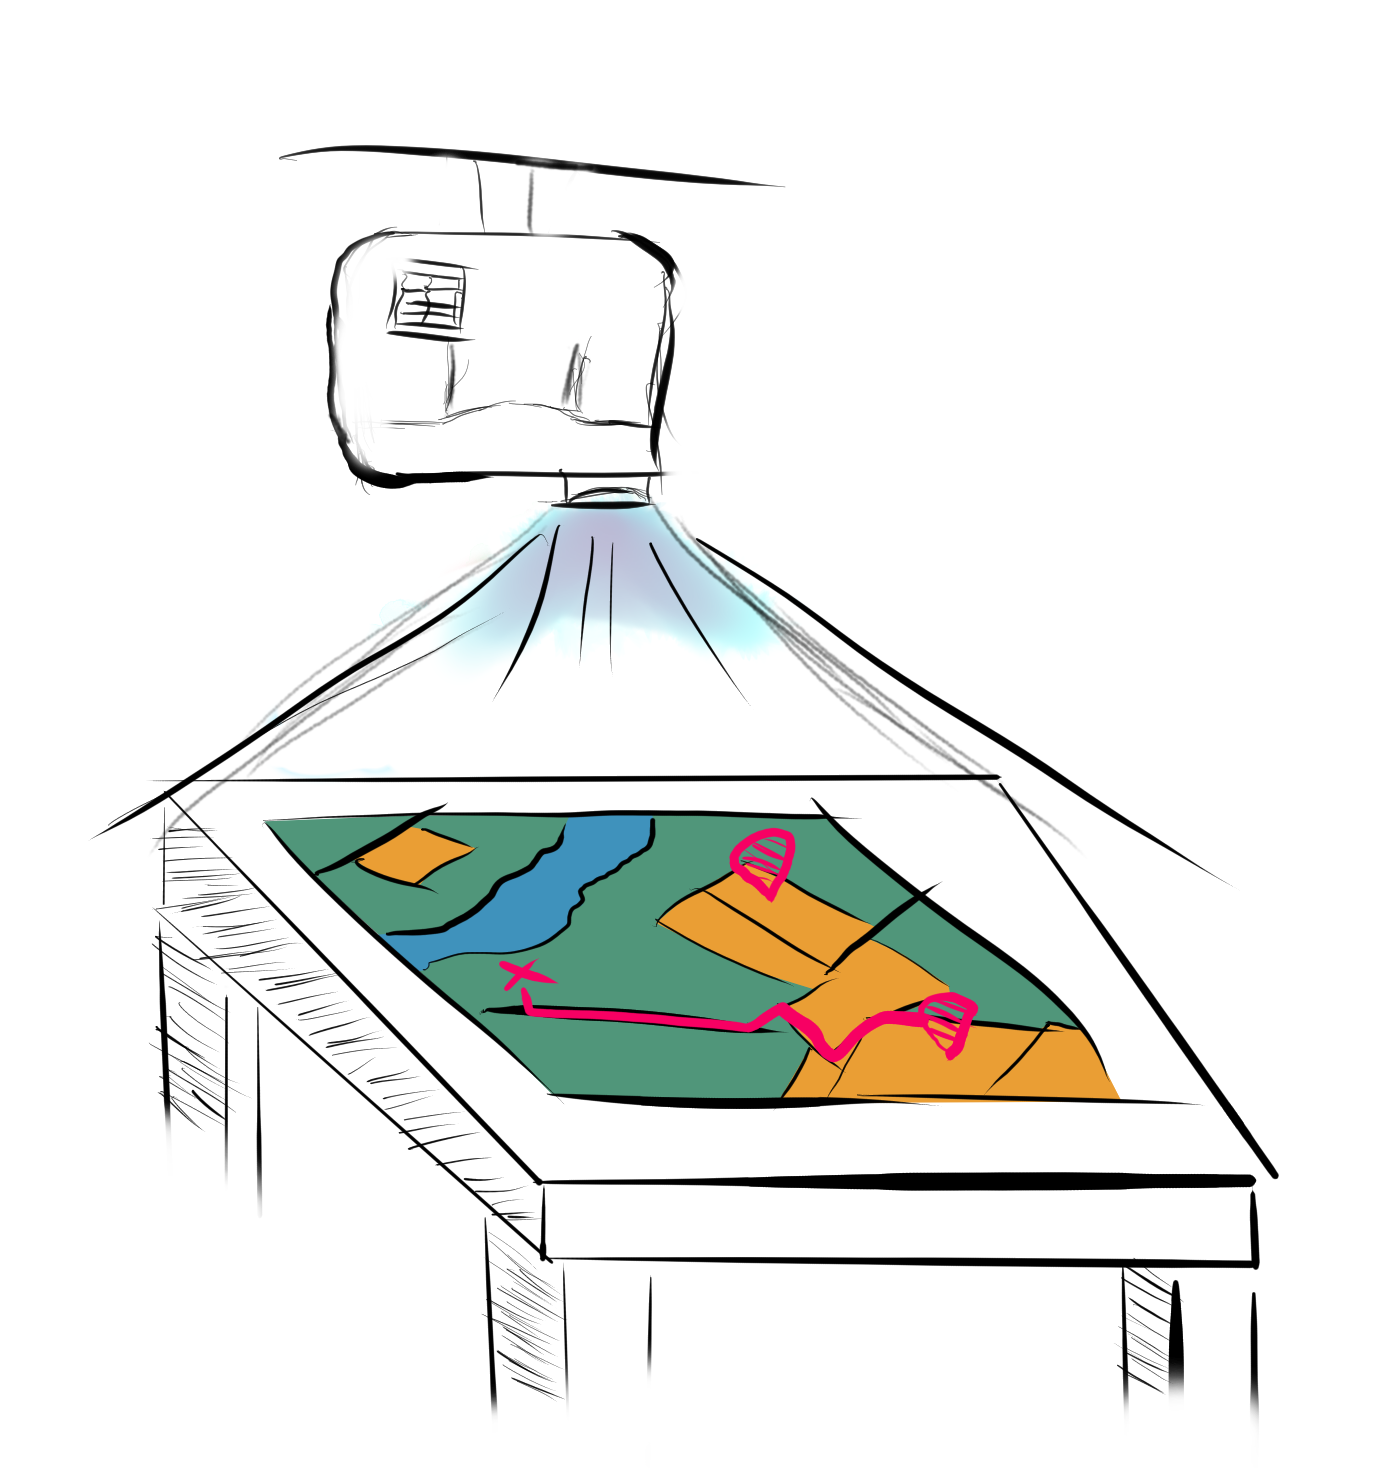
\includegraphics[height=0.4\textheight]{figures/sketch_ar_projected}
        \hfill
    }
    \caption{Kategorie 4: Mit Projektoren werden digitale Inhalte (hier \textcolor{magenta}{Magenta}) auf reale Objekte und Oberflächen projiziert.}
    \label{fig:sketch_ar_projected}
\end{figure}

Die letzte Kategorie umfasst Spatial AR Arbeiten, die projizierende Technologien nutzen, um digitale Navigationsinformationen direkt auf physischen Oberflächen anzuzeigen.

Dazu zählt der Ansatz von \textcite{Reitmayr2005}, bei dem eine reale Papierkarte durch einen Projektor augmentiert wird.
\autoref{fig:reitmayr2005_helicopter_map} zeigt die Funktionsweise.
Ein projizierter Helikopter kann mit einem realen \emph{Personal Digital Assistant} (PDA) bewegt werden, wenn dieser in die Nähe gehalten wird.
Der PDA zeigt währenddessen ein Interface zur Kontrolle des Helikopters.
Der Helikopter dient als Cursor für kontextbasierte Informationen.
Sobald der Nutzer einen Rahmen auf die Karte legt, projiziert der Projektor ein Bild der aktuellen Kartenposition aus ungefährer Sicht des Helikopters auf ihn.
Zudem kann der Zustand der Karte durch die Projektion dynamisch verändert werden (in diesem Fall werden Gezeiten von Gewässern simuliert).
Die Arbeit verdeutlicht, dass mit AR nicht nur ortsbezogene sondern auch zeitbezogene Daten auf einer Karte dargestellt werden können.
Dies erlaubt eine Exploration in der zeitlichen Dimension einer Karte.

\textcite{Roo2017} präsentieren einen augmentierten Zen-Garten (siehe \autoref{fig:roo2017_sandbox_island}).
Sie projizieren die Übersichtskarte einer Insel auf einen Sandkasten, wobei die Insel abhängig ist von der Anhäufung des Sands.
Die unterschiedlichen Regionen (Wasser, steiles oder flaches Gelände, Wald) werden durch unterschiedliche Farben des projizierten Lichts hervorgehoben.
Über einen physischen Avatar kann der Nutzer eine dreidimensionale Variante der Insel über ein VR-HMD betreten.
Dieser Ansatz verdeutlicht, dass ein Spatial-AR-Interface auch genutzt werden kann, um in einer rein virtuellen Umgebung zu navigieren.

\begin{figure}[h]
\begin{minipage}[t]{0.48\textwidth}
    \centering
    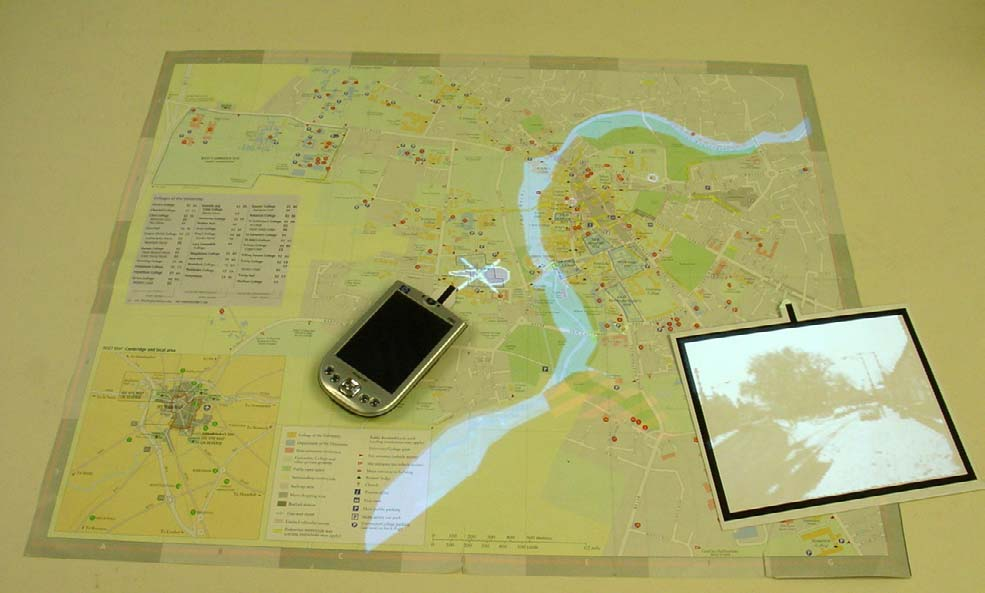
\includegraphics[width=\textwidth, height=0.25\textheight]{figures/reitmayr2005_helicopter_map}
    \caption{Eine reale Papierkarte wird durch einen Projektor mit virtuellen Inhalten angereichert. \quelle{\cite{Reitmayr2005}}}
    \label{fig:reitmayr2005_helicopter_map}
\end{minipage}%
\hfill
\begin{minipage}[t]{0.48\textwidth}
    \centering
    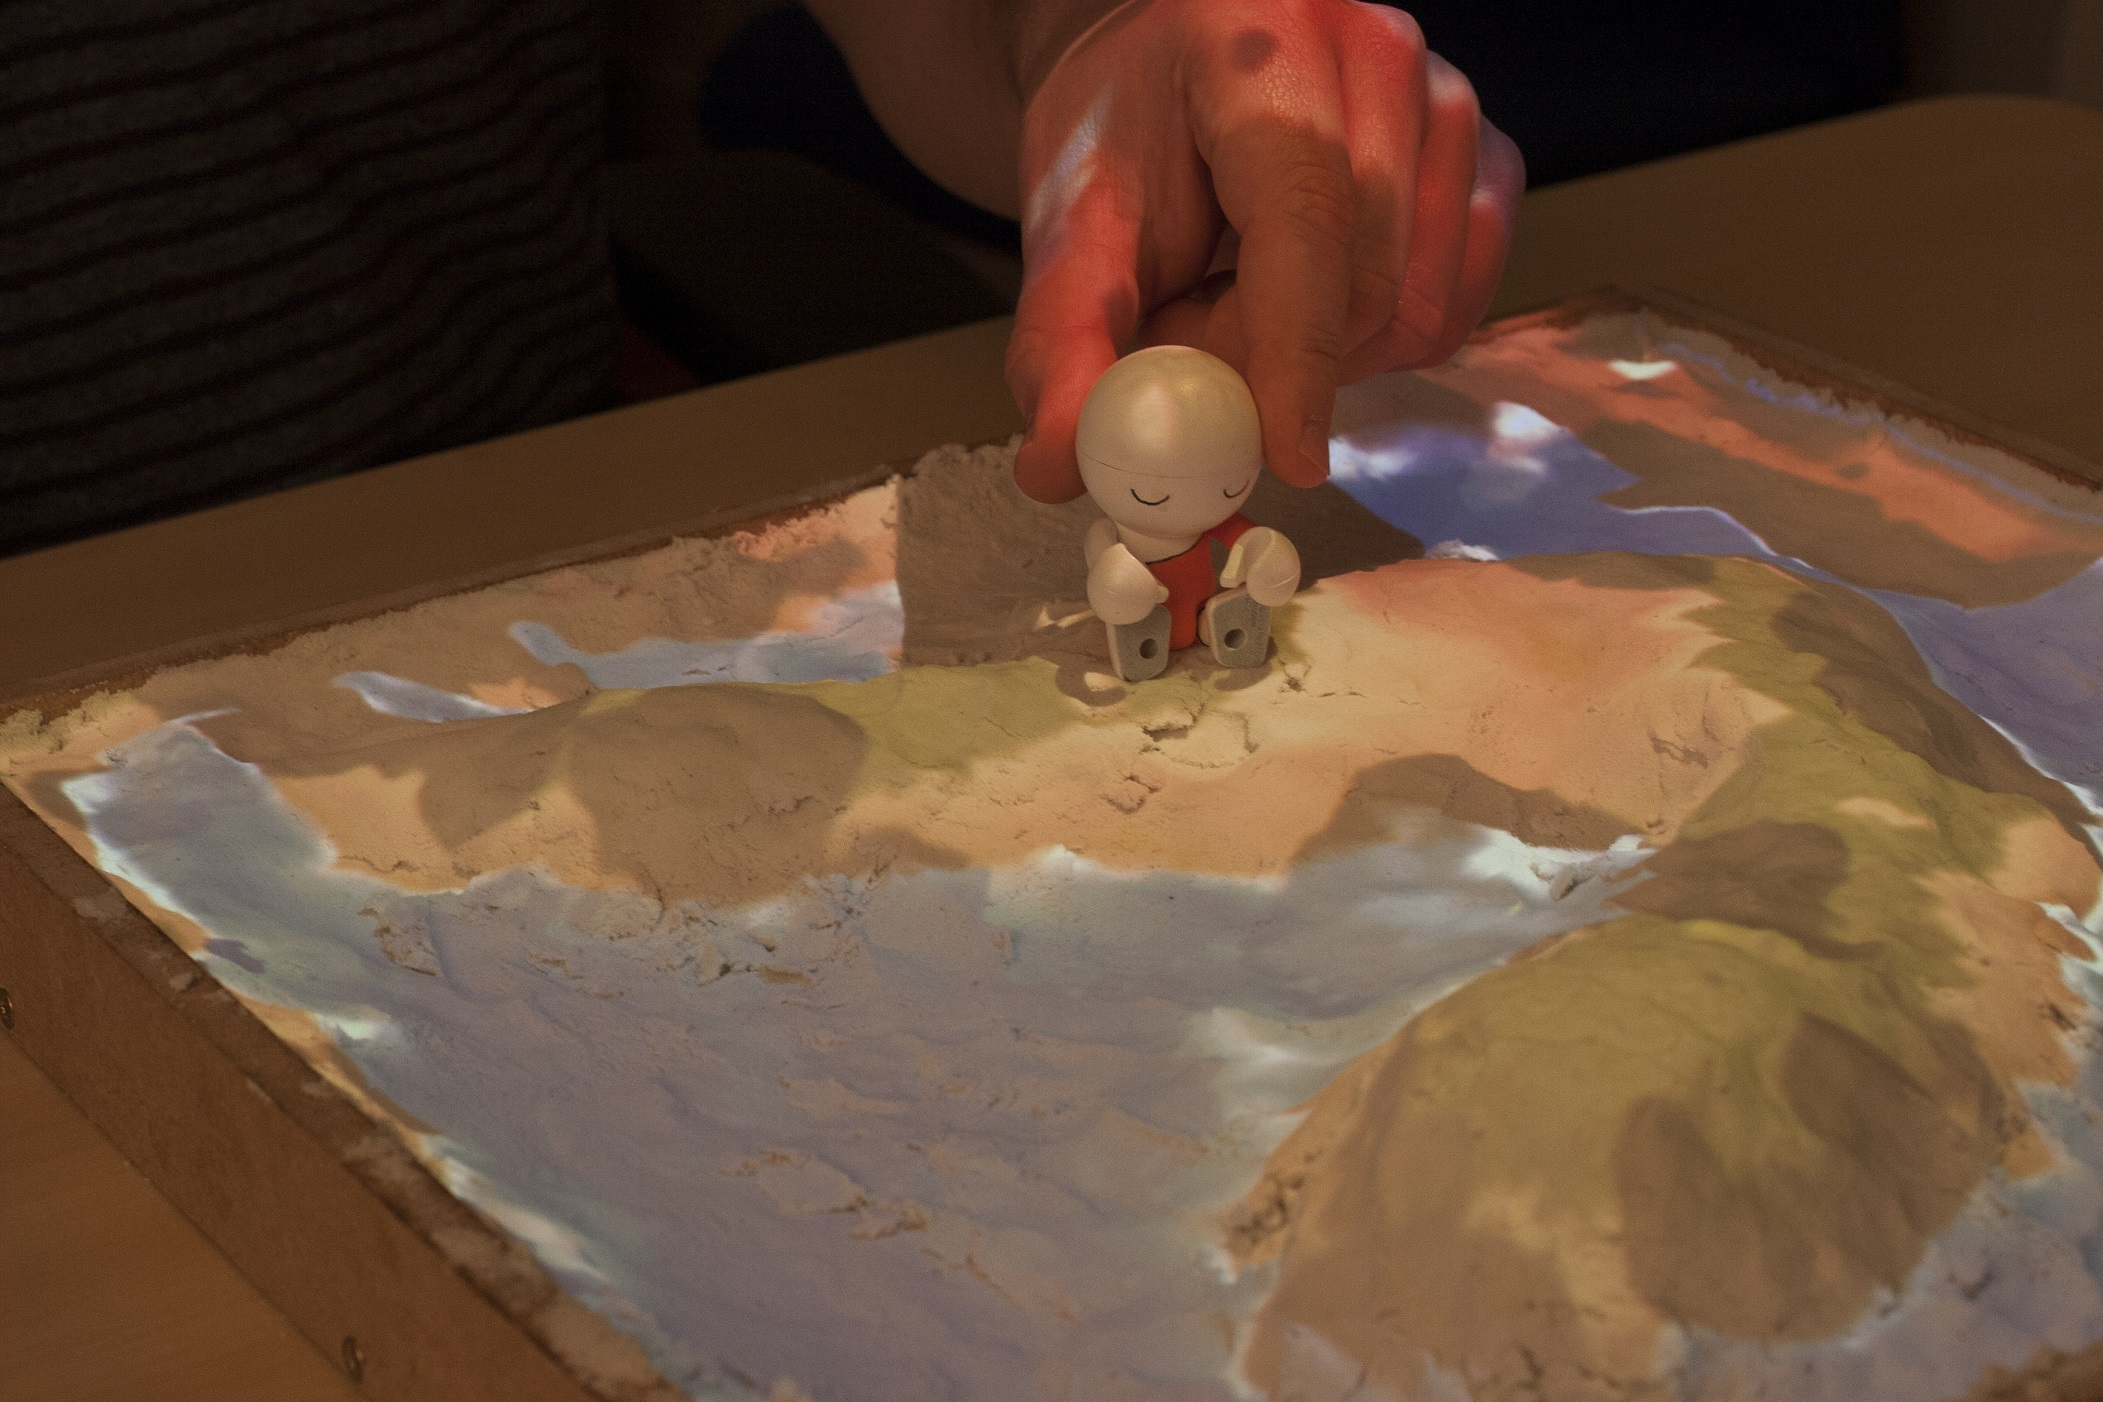
\includegraphics[width=\textwidth, height=0.25\textheight]{figures/roo2017_sandbox_island}
    \caption{Ein physischer Avatar erlaubt dem Nutzer, seine Position in der dazugehörigen virtuellen Umgebung zu ändern. \quelle{\cite[1462]{Roo2017}}}
    \label{fig:roo2017_sandbox_island}
\end{minipage}
\end{figure}

Bei dieser Methode sind die Hände frei, was Nutzern die Interaktion mit der Umgebung erlaubt.
Da hier die Umgebung \emph{selbst} als Display dient, ermöglicht diese Herangehensweise taktiles Feedback für die Nutzer wenn diese mit Objekten in der Umgebung interagieren.
Da Nutzer außerdem keine separate Displaytechnologie verwenden, ist ihr natürliches Blickfeld (\emph{Field-of-View}, FOV) nicht eingeschränkt.
Ein begrenztes FOV würde die Immersion verringern, was hier nicht der Fall ist \parencite[3\pageff]{Krevelen2010}. % TODO: cite!

Die Methode der Projektion wird jedoch durch das Umgebungslicht beeinflusst.
In einer hell erleuchteten Umgebung sind die Projektionen schlechter zu erkennen \parencite{???} % TODO: cite!
Ein weiteres Problem ist das Verdecken durch dynamische Objekte.
Wie in \autoref{fig:roo2017_sandbox_island} zu sehen ist werden die virtuellen Inhalte auf die Arme und Hände projiziert, sobald sich diese über dem Sandkasten befinden.
Außerdem können die Karten nicht nach Belieben gezoomt werden.
Zum Beispiel kann die Größe der Karte aus \autoref{fig:reitmayr2005_helicopter_map} während der Nutzung nicht angepasst werden, wodurch sich der Detailgrad der zugrundeliegenden Karte nicht ändern lässt.

\section{Navigation und Exploration in digitalen Spielen}
Wie in \autoref{sec:motivation_ziel} erwähnt nehmen Navigation und Exploration eine wichtige Rolle in digitalen Spielen ein.
\textcites{Moura2014}{Moura2015} untersuchen den Zusammenhang zwischen eingesetzten Navigationshelfern, Design der Level, sowie Spielmechaniken zur Unterstützung der Navigation.
Daraus leiten \textcite{Moura2015} eine Klassifikation von Navigationshelfern ab.
Außerdem erstellen sie eine Liste von Design-Richtlinien, welche die Vor- und Nachteile der jeweiligen Helfer erläutern und als Hilfestellung für Entwicklung von neuen Spielen dienen.
Diese Designrichtlinien werden in die Entwicklung der Megamap mit einbezogen.

Aufbauend auf die Navigationshelfer in Spielen untersucht \textcite{Lodts2015}, ob diese Helfer auch in der realen Welt anwendbar sind.
Dazu wurden unterschiedliche Helfer, wie sie aus Spielen bekannt sind, für das \emph{Google Glass} implementiert.
In einem Test, aufgeteilt in die Aufgabenbereiche Navigation, Orientierung, Exploration und Annotation, wurde ermittelt welche der Helfer den Nutzern bei der jeweiligen Aufgabe am hilfreichsten sind.
Es zeigt sich, dass Helfer, die in der Umgebung eingebettet sind (z.B. AR-Pfeile oder -Text, farbliche Hervorhebungen von Objekten) effektiver sind als statische Anzeigen per \emph{Head-Up Display} (HUD).
Dies spricht für den Ansatz dieser Arbeit, eine Karte in die Umgebung des Nutzers zu integrieren.

\section{Beitrag dieser Masterarbeit}
Diese Arbeit hebt sich in zwei Aspekten vom bisherigen Stand der Forschung ab.
Zum einen wird eine Kartenanwendung speziell für ein VR-HMD entwickelt.
Dadurch kann die Karte direkt in die (virtuelle) Umgebung des Nutzer eingebettet werden.
Die Verwendung des Stereodisplays im HMD erweitert die Tiefenwahrnehmung der Nutzer, was für die Betrachtung der komplexen mehrstöckigen Innenstrukturen von Gebäuden hilfreich ist \parencite[vgl.][]{Rantakari2017}.
Die Implementierung für ein VR-HMD kann als Sprungbrett für zukünftige Arbeiten betrachtet werden, die das gleiche Konzept für MR-HMDs umsetzen könnten, bei denen die Karte in die \emph{reale} Umgebung des Nutzers integriert wird.
In \autoref{chap:closing} wird näher auf die Herausforderungen bei einer Umsetzung für MR-HMDs eingegangen.

Zum anderen wird der Anwendungsfall der Indoor-Kartenexploration näher beleuchtet.
Wie zu sehen ist setzen sich die bisherigen Ansätze im Bezug auf Indoor-Orte meistens nur mit der reinen Navigation oder Lokalisierung auseinander.
Diese Arbeit fokussiert hingegen die Karten\emph{exploration}.
Zu diesem Zweck wird analysiert, wie bereits existierende Kartenanwendungen das Erkunden der Umgebung vereinfachen.
Dabei beschränkt sich die Analyse nicht nur auf Indoor-Anwendungen, sondern bezieht auch Outdoor-Anwendungen (z.B. Google Maps) oder gar digitale Spiele mit ein.
Schließlich werden die hieraus gewonnenen Erkenntnisse auf den Indoor-Einsatz übertragen und prototypisch implementiert.
%
\cleardoublepage
